\section{Installations- und Bedienungsanleitung}
\microtypesetup{expansion=false}
\subsection{Zielgruppe und Zweck}

Diese Anleitung richtet sich an technische Nutzer:innen (Tutor:innen, Reviewer, Entwickler:innen),
die das System lokal in Betrieb nehmen, testen und demonstrieren möchten.
Sie beschreibt die Inbetriebnahme und Bedienung der folgenden Komponenten:

\begin{itemize}
  \item Backend (Spring Boot, REST-API) inkl.\ Datenbank via Docker
  \item Android-App (Kotlin / Jetpack Compose)
  \item Web-Anwendung (Web-GUI, Anbindung an das Backend über REST)
  \item Optional: Smartwatch / Wear~OS (Datenquelle / Synchronisation)
\end{itemize}


\subsection{Rollen und Berechtigungen (Kurzüberblick)}

\begin{itemize}
  \item \textbf{Patient (PATIENT):} Erstzugang über Einladungs- bzw.\ Zugangscode,
        Erfassung eigener Daten, kein Zugriff auf fremde Daten.
  \item \textbf{Arzt/Ärztin (ARZT):} Anmeldung mit bereitgestelltem Konto,
        Erstellung von Zugangscodes, Zugriff nur auf zugewiesene Patient:innen,
        Auswertung und Report-Erstellung.
\end{itemize}


\subsection{Voraussetzungen (Software)}

\begin{itemize}
  \item \textbf{Docker Desktop} inkl.\ Docker Compose (Datenbank)
  \item \textbf{Java JDK~17}
  \item \textbf{Android Studio} (für die Android-App)
  \item \textbf{Visual Studio Code} (für die Web-Komponente)
\end{itemize}

\clearpage

%-----------------------------------------------------------

\subsection{Backend: Infrastruktur und Server starten}

\textbf {Start der Datenbank und abhängiger Services in Docker-Containern.}

\begin{enumerate}
  \item Docker Desktop öffnen und sicherstellen, dass Docker läuft
        (Status: \emph{running}).
  \item Terminal öffnen und ins Projektverzeichnis wechseln:
\begin{verbatim}
cd <pfad-zum-repo>/src/back
\end{verbatim}
  \item Container starten:
\begin{verbatim}
docker compose up -d
\end{verbatim}
\end{enumerate}

\textbf{Erwartetes Ergebnis:}
\begin{itemize}
  \item Container laufen stabil ohne Crash (sichtbar in Docker Desktop).
  \item Datenbank ist erreichbar.
\end{itemize}

\begin{figure}[h]
  \centering
  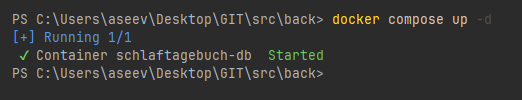
\includegraphics[width=0.9\textwidth]{images/anleitung/docker.png}
  \caption{Erfolgreicher Start der Datenbank über Docker Compose}
  \label{fig:db}
\end{figure}

\smallskip

\textit{Datenbank prüfen (optional)}
\textbf{Variante A: Docker Desktop}
\begin{itemize}
  \item Running Containers $\rightarrow$ Datenbank-Container $\rightarrow$ Logs prüfen (keine Crash-Loops).
\end{itemize}

\textbf{Variante B: DB-Client (IntelliJ Database / pgAdmin)}
\begin{itemize}
  \item Host: \texttt{127.0.0.1}
  \item Port: \texttt{5433}
  \item Credentials: gemäß \texttt{docker-compose.yml} / \texttt{.env}
  \item Erwartung: Tabellen/Schemata sind sichtbar.
\end{itemize}
\bigskip

%---------------------------------------------------------------

\textbf{REST-API lokal starten}

\begin{enumerate}
  \item Terminal im Backend-Verzeichnis öffnen.
  \item Server starten:
\begin{verbatim}
.\gradlew bootRun
\end{verbatim}
  (nachdem die Datenbank mit \texttt{docker compose up -d} gestartet wurde)
  \item Alternativ: Start über IDE (Run-Konfiguration).
\end{enumerate}

\textbf{Erwartetes Ergebnis (Erfolgsindikatoren):}
\begin{itemize}
  \item Im Terminal erscheinen Hibernate-Logausgaben (z.\,B. SQL-Selects auf die Tabelle \texttt{user\_account}) sowie der Status \texttt{EXECUTING :bootRun}.
  \item Es treten keine roten Stacktraces oder Abbruchmeldungen auf.
  \item Der Prozess bleibt aktiv und wartet auf eingehende Requests.
\end{itemize}

\textbf{Hinweis:}  
Die angezeigten Hibernate-Abfragen sowie der laufende \texttt{bootRun}-Prozess zeigen, dass das Backend erfolgreich gestartet ist und betriebsbereit ist. Der Gradle-Fortschritt verbleibt typischerweise bei ca. 80\,\%.

\begin{figure}[h]
  \centering
  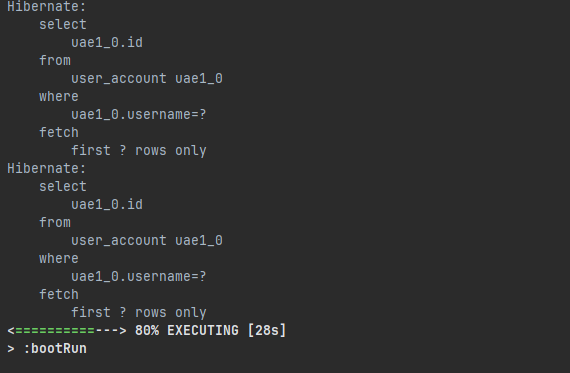
\includegraphics[width=0.9\textwidth]{images/anleitung/back.png}
  \caption{Erfolgreicher Start des Backends mit laufendem \texttt{bootRun}-Prozess}
  \label{fig:bootrun}
\end{figure}

\textbf{Überprüfung der Funktionsfähigkeit:}
\begin{itemize}
  \item Eine Überprüfung über den Webbrowser ist nicht möglich, da das Backend ausschließlich REST-Endpunkte bereitstellt.
  \item Die Funktionsfähigkeit kann entweder über ein API-Testtool (z.\,B. Postman) oder über die angebundenen Frontends (Android-App oder Web-GUI) überprüft werden.
\end{itemize}

\newpage

% --------------------------------------------------

\subsection{Web-Anwendung}

\begin{enumerate}
  \item Visual Studio Code öffnen.
  \item Extension \emph{Live Server} installieren.
  \item Web-Ordner öffnen (\texttt{src/HTML} ).
  \item \texttt{login.html} öffnen.
  \item Rechtsklick $\rightarrow$ \emph{Open with Live Server}.
\end{enumerate}

\textbf{Erwartetes Ergebnis:}
\begin{itemize}
  \item Browser öffnet eine lokale URL (z.\,B. \texttt{http://127.0.0.1:5500/}).
  \item Seite wird korrekt gerendert, keine 404 im Browser.
\end{itemize}

\smallskip

\textit{Authentifizierungspfad prüfen.}

\begin{enumerate}
  \item \textbf{Login-Seite:} Benutzername/Passwort eingeben 
  \\ (Benutzername: arzt1, Passwort: arztpass) 
  \\ $\rightarrow$ erfolgreicher Übergang zur Hauptübersicht.
  \item \textbf{Navigation:} Über Sidebar sind alle anderen Seiten zu erreichen $\rightarrow$ "Abmelden" um zur Login-Seite zu kommen.
  \item \textbf{Hauptübersicht:} Anzahl der Patient:innen und Berichte, die zur Verfügung stehen sowie letzte Aktivitäten einsehen.
  \item \textbf{Patient:innen-Seite:} Patientendaten beinhalten Geburtsdatum, Zugangscode, Termin und Bericht.
  \item \textbf{Zugangscodes-Seite:} Erstellung von Zugangscode (Voraussetzung: Patient gewählt, Gültigkeitsdatum gewählt, Termin gewählt).
  \item \textbf{Berichte-Seite:} Nach 14 Tagen können hier Berichte von Patient:innen im PDF-Format heruntergeladen werden.
\end{enumerate}
\newpage

% --------------------------------------------------
\subsection{Android: App starten und Grundfunktion prüfen}

\textbf{Variante A: Emulator}
\begin{enumerate}
  \item Android Studio $\rightarrow$ \emph{Device Manager}.
  \item Emulator erstellen (z.\,B. Pixel-Gerät, Android-Version gemäß Projektvorgaben).
  \item Emulator starten.
\end{enumerate}

\textbf{Variante B: Physisches Gerät}
\begin{enumerate}
	\item Auf dem Android-Gerät die Entwickleroptionen aktivieren (in den Einstellungen 7x auf \glqq Build-Nummer\grqq{} tippen z.B. unter Einstellungen/ Telefoninfo/ Softwareinformation/ Buildnummer).
	\item In den Entwickleroptionen \textbf{USB-Debugging} aktivieren.
	\item Gerät via USB mit dem PC verbinden und den RSA-Fingerprint (angezeigt Meldung) bestätigen.
	\item In Android Studio im Dropdown-Menü das physische Gerät auswählen.
\end{enumerate}

\textbf{In Android-Studio:}

\begin{enumerate}
  \item Das App-Modul auswählen.
  \item Zielgerät wählen (Emulator oder physisches Gerät).
  \item \emph{Run} starten.
\end{enumerate}

\textbf{Erwartetes Ergebnis:}
\begin{itemize}
  \item App wird installiert und startet ohne Crash.
  \item Sprache-/Login-Screen/Menü erscheint.
\end{itemize}

\textbf{Nachweis:} Screenshot vom Start-/Login-Screen (Abb. \_\_) und ggf. Logcat-Ausschnitt ohne Fehler.

\medskip

\textbf{Authentifizierungspfad prüfen.}

\begin{itemize}
  \item \textbf{Patient First Login:} Die Sprache auswählen $\rightarrow$ Konto erstellen $\rightarrow$ Einladungscode eingeben und PbD eingeben (und ggf. Zusatzdaten) $\rightarrow$ Account-Aktivierung $\rightarrow$ Hauptansicht.
  
  \item \textbf{Einstellungen verwalten:} Menü $\rightarrow$Knopf mit  Einstellungen $\rightarrow$ $\rightarrow$ Änderung vornehmen (z.\,B. Erinnerungszeit) $\rightarrow$ Zurück zur Hauptansicht (Änderung ist gespeichert).

  \item \textbf{Smartwatch koppeln:} Bluetooth Einstellungen $\rightarrow$ Falls Smartwatch nicht angezeigt dannn Geräte suchen $\rightarrow$ Mit Smartwatch verbinden $\rightarrow$ App auf der Smartwatch öffnen $\rightarrow$ Gibt Feedback bei Schlaf Starten.

  \item \textbf{Protokoll ausfüllen:} Menü $\rightarrow$ Knopf mit Fragebogen starten $\rightarrow$ Fragen mit weiter durchklicken

  \item \textbf{Bericht ansehen:} Menü $\rightarrow$ Button mit Bericht herunterladen (PDF) $\rightarrow$ Es öffnet sich eine PDF (oder Fehler weil kein Server)
\end{itemize}

\textbf{Erwartetes Ergebnis:}
\begin{itemize}
  \item Erfolgreiche Anmeldung führt zur jeweiligen Hauptansicht.
  \item Bei ungültigen Eingaben erscheint eine verständliche Fehlermeldung.
\end{itemize}
\bigskip

% --------------------------------------------------
\subsection{Smartwatch / Wear OS (optional)}

\textbf{Variante A: Wear OS Emulator}
\begin{enumerate}
  \item Android Studio $\rightarrow$ \emph{Device Manager}.
  \item Wear OS Emulator erstellen und starten.
\end{enumerate}

\textbf{Variante B: Physische Smartwatch}
\begin{enumerate}
  \item Auf der Smartwatch: \textbf{Entwickleroptionen} aktivieren (Einstellungen $\rightarrow$ System $\rightarrow$ Info $\rightarrow$ 7x auf \glqq Build-Nummer\grqq{} tippen).
  \item In den Entwickleroptionen \textbf{ADB-Debugging} und \textbf{Debugging über WLAN} aktivieren.
  \item In Android Studio: \emph{Device Manager} öffnen $\rightarrow$ \emph{Pair using Wi-Fi}.
  \item Den Anweisungen auf Uhr und PC folgen (QR-Code scannen oder Code eingeben).
\end{enumerate}

\textbf{Erwartetes Ergebnis:}
\begin{itemize}
  \item Wearable wird erkannt.
  \item Synchronisation kann angestoßen werden (falls implementiert).
\end{itemize}

\textbf{Nachweis:} Screenshot der Wear-Ansicht oder Logcat-Eintrag der Synchronisation (Abb. \_\_).

\newpage
\section{Quellenangabe (Informationsbeschaffung / Dokumentation)}

Die folgende Liste enthält die im Rahmen des Projekts verwendeten offiziellen Dokumentationen und Ressourcen zur Informationsbeschaffung.

\begin{itemize}

  \item \textbf{Android / Mobile App}
  \begin{itemize}
    \item Jetpack Compose – Offizielle Dokumentation: \\
    \url{https://developer.android.com/compose}
    \item Material Design 3 – Komponenten: \\
    \url{https://m3.material.io/components}
  \end{itemize}

  \item \textbf{Backend / Server}
  \begin{itemize}
    \item Spring Boot – Offizielle Dokumentation: \\
    \url{https://spring.io/projects/spring-boot}
  \end{itemize}

  \item \textbf{Datenbank}
  \begin{itemize}
    \item PostgreSQL – Offizielle Dokumentation: \\
    \url{https://www.postgresql.org/docs/}
  \end{itemize}

  \item \textbf{Containerisierung}
  \begin{itemize}
    \item Docker – Offizielle Dokumentation: \\
    \url{https://docs.docker.com/}
  \end{itemize}

  \item \textbf{API-Tests}
  \begin{itemize}
    \item Postman – Offizielle Dokumentation: \\
    \url{https://learning.postman.com/}
  \end{itemize}

  \item \textbf{Web-Technologien}
  \begin{itemize}
    \item HTML – Dokumentation: \\
    \url{https://www.w3schools.com/html/}
    \item JavaScript – Dokumentation: \\
    \url{https://www.w3schools.com/js/}
    \item CSS – Grundlagen (SelfHTML Wiki): \\
    \url{https://wiki.selfhtml.org/wiki/CSS}
  \end{itemize}

\end{itemize}

\newpage

\subsection{Verwendete Tools und Programme}

Im Rahmen des Projekts wurden folgende Tools und Programme eingesetzt:

\begin{itemize}

  \item \textbf{Entwicklung und Programmierung}
  \begin{itemize}
    \item Android Studio
    \item IntelliJ IDEA
    \item Visual Studio Code
  \end{itemize}

  \item \textbf{Versionsverwaltung}
  \begin{itemize}
    \item Git \\
    \url{https://git-scm.com}
    \item GitLab (Repository und CI/CD)
  \end{itemize}

  \item \textbf{Backend und Infrastruktur}
  \begin{itemize}
    \item Spring Boot
    \item Docker
    \item PostgreSQL
    \item Gradle
  \end{itemize}

  \item \textbf{API-Tests}
  \begin{itemize}
    \item Postman
  \end{itemize}

  \item \textbf{Diagramme und Dokumentation}
  \begin{itemize}
    \item draw.io (Diagrammerstellung) \\
    \url{https://app.diagrams.net}
    \item Affinity Publisher (Layout und PDF-Erstellung) \\
    \url{https://www.affinity.serif.com/de/publisher/}
    \item LaTeX \\
    \url{https://www.latex-project.org/help/documentation/}
  \end{itemize}

  \item \textbf{Medien und Präsentation}
  \begin{itemize}
    \item Clipchamp (Video-Editing) \\
    \url{https://clipchamp.com/de/video-editor/}
  \end{itemize}

\end{itemize}